\section{Experimental Evaluation}
\label{sec:eval}
The evaluation examines three evidence layers of the operation path: configured signal mappings, application-level governance routes, and subsequent process observations. We first test mappings and limits through selected direct API requests, then report an exploratory simulator contrast between a scripted setpoint policy and a no-write condition. Separate fixtures examine guard and approval-route responses. An injection-twin run and three LLM-driven episodes are non-evaluative follow-up observations rather than complete agent-to-device trials. These blocks use different test units and evidence sources. Integrated checks used already-running platform and simulator services, generally in benchmark mode, which bypasses step, interval, and hold-window checks for agent or manual writes. Individual ablation configurations also removed selected checks. No cold-start deployment or physical-plant run was performed.

A service response, a simulated readback, and a later process measurement are distinct. An accepted request does not by itself establish driver dispatch, and a later process value does not identify the write that caused it.

\subsection{Configured Mapping and Integration Checks}
\label{sec:eval-mapping}
Two integrated executions, both with seed~42, each passed 77 assertions across 17 phases. Both began with the platform and simulator already running, and neither activated an agent harness. A film-line preset check configured five endpoint types and rejected nine selected negative probes; it reused the same runtime and is not an independent deployment replication. These runs therefore assess direct runtime/API behavior, not the complete task-mediated path described in the architecture.

The scene--protocol probes covered 55 configured write-capable endpoints in four simulated scenes using Modbus Transmission Control Protocol (TCP), Modbus remote terminal unit (RTU), OPC Unified Architecture (OPC UA), Message Queuing Telemetry Transport (MQTT), and Hypertext Transfer Protocol (HTTP). Table~\ref{tab:scene-probe-results} gives the scene-level counts. The probe plan specified three requests for interior values, one for the upper boundary, and four for values outside the structural range at each endpoint. All 220 requests with prespecified admissible values received the expected acceptance response; all 219 collected out-of-range requests received the expected rejection, and all 216 available simulator readbacks matched. These probes assess selected mappings; the tested values and guards derive from the same configured limits. One structural request was not collected; HTTP endpoints do not expose readback, and the scene--protocol matrix is incomplete.

\begin{table*}[!t]
\centering
\caption{Configured scene--protocol probes. Counts show prespecified admissible requests receiving the expected acceptance response, out-of-range requests receiving the expected rejection, and matching simulator readbacks where supported.}
\label{tab:scene-probe-results}
\footnotesize
\setlength{\tabcolsep}{3pt}
\begin{tabularx}{\textwidth}{@{}>{\raggedright\arraybackslash}p{1.55cm}r X r r r@{}}
\toprule
Scene & Configured endpoints & Protocols represented & Accepted probes & Structural rejects & Simulator readbacks \\
\midrule
Injection & 11 & TCP 5; RTU 2; OPC UA 3; MQTT 1 & 44/44 & 44/44 & 44/44 \\
Wastewater & 7 & TCP 1; RTU 3; OPC UA 2; MQTT 1 & 28/28 & 28/28 & 28/28 \\
Annealing & 7 & TCP 3; RTU 2; OPC UA 1; MQTT 1 & 28/28 & 28/28 & 28/28 \\
Biaxial line & 30 & TCP 20; RTU 1; OPC UA 8; HTTP 1 & 120/120 & 119/119 & 116/116 \\
\bottomrule
\end{tabularx}
\end{table*}

\subsection{Exploratory Fixed-Horizon Simulator Contrast}
\label{sec:eval-optimization}
We compared a deterministic bounded setpoint policy with a no-write condition in injection, wastewater, and annealing simulations. The policy used the \texttt{recipe\_trial} route. The available candidate policy adjusts injection holding pressure and time, wastewater blower and dosing settings, and annealing-zone temperatures and line speed according to scene-specific conditions. The target bands were $32.5\pm0.35$~g for part weight, $3.4\pm0.6$~mg/L for dissolved oxygen, and $95\pm6$~HV for hardness, respectively. Each scene used its own fixed horizon (180~s for injection; 240~s for the other scenes), nominal one-second sampling, an independent reset for each arm, and a pre-specified initial-process-value window. Arm order was randomized within each scene--seed block, but paired starts were not required to have identical process values. The primary outcome was integrated absolute error (IAE), the time integral of the absolute deviation from the target, calculated by the trapezoidal rule over the retained samples between the first and last retained points. Internal gaps up to 5~s were linearly interpolated; no extrapolation was made to the nominal window endpoints, and a larger gap invalidated the pair.

In the later batch of 11 post-pilot scene--seed blocks, nine met the reset, initial-window, and sampling rules. Two blocks (wastewater seed~45 and annealing seed~46) were invalid because their no-write traces had 9-s and 6-s gaps. An earlier batch also contains an independently reset, valid injection seed-44 block with $\Delta\mathrm{IAE}=193.320$~g\,s; the later batch repeated that block and yielded 165.165~g\,s. The available records do not establish a rule for selecting between batches; the earlier batch also contains failed reset attempts. The reported subset is therefore exploratory and cannot be treated as a complete, non-repeated set of attempted blocks. Every valid block in the later batch had a positive $\Delta\mathrm{IAE}=\mathrm{IAE}_{\mathrm{no\text{-}write}}-\mathrm{IAE}_{\mathrm{scripted}}$. Among the valid blocks, recorded samples from every scripted run entered its target band, whereas none from the no-write runs did. Table~\ref{tab:selected-iae} reports per-scene medians and ranges; the complete selected-batch records, invalid blocks, earlier block, and exclusion rationale are provided in Supplementary File~S7 and the accompanying evidence archive.

\begin{table}[!t]
\centering
\caption{Selected fixed-horizon simulator contrasts. Positive $\Delta$IAE means lower retained-window accumulated absolute error under the scripted policy.}
\label{tab:selected-iae}
\footnotesize
\setlength{\tabcolsep}{3pt}
\begin{tabular}{@{}lcc@{}}
\toprule
Scene (unit of $\Delta$IAE) & Valid & Median (range) \\
\midrule
Injection (g\,s) & 3/3 & 165.165 (162.535--195.169) \\
Wastewater ((mg/L)\,s) & 3/4 & 615.605 (611.670--630.980) \\
Annealing (HV\,s) & 3/4 & 8000.450 (7930.200--8084.150) \\
\bottomrule
\end{tabular}
\end{table}

The unresolved batch-selection rule limits inference from these results. The sample is small, simulator seeds are not independent plants, and no proportional--integral--derivative or model-predictive-control baseline was tested. The run record reports a combined SHA-256 matching local copies of the paired-run and scene-policy scripts. This self-reported hash does not independently establish the executed process image, and a complete service and simulator snapshot was not identified. The archive therefore does not support full end-to-end reproduction. Accordingly, we make no significance or broad efficacy claim.

Fig.~\ref{fig:optimization-trajectory}(a) shows the mass traces for the three valid injection blocks, and Fig.~\ref{fig:optimization-trajectory}(b) tabulates their recorded setpoint requests. For each scripted mass trace, a recorded sample entered the target band within the first 15~s; subsequent samples fluctuated near its lower boundary, whereas the no-write traces stayed near their initial values. The task logs report a 31.2~g baseline, which need not equal the first sample in the plotted horizon. Seeds~44 and~45 each recorded a pressure request followed by a hold-time request; seed~46 recorded a further pressure request (58$\rightarrow$61.88~bar) after its hold-time request. The task script's final post-settling means were 32.163, 32.190, and 32.383~g, respectively, within the 32.15--32.85~g band. The starting and requested values in Fig.~\ref{fig:optimization-trajectory}(b) are script records, not independent device readbacks. For seed~46, a prior request to 57.97~bar and a later recorded starting value of 58~bar are shown as recorded. The archive neither aligns requests with acquisition timestamps nor preserves a per-request server ledger. Fig.~\ref{fig:optimization-trajectory}(c)--(e) compare IAE for the nine selected blocks by scene; Table~\ref{tab:selected-iae} reports the contrasts.

\begin{figure*}[!t]
\centering
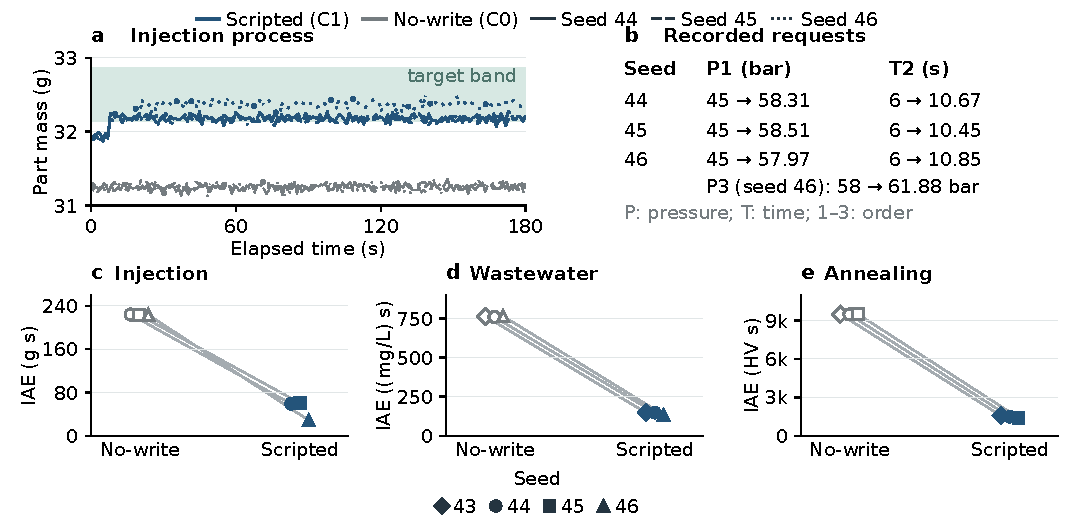
\includegraphics[width=\textwidth]{resources/fig5.pdf}
\caption{Selected simulator observations. (a) Recorded part-mass samples for the three valid injection scene--seed blocks over the nominal 180~s window; the shaded band is 32.15--32.85~g. Color distinguishes no-write (C0) from the scripted policy (C1), and line style identifies the seed. Sampling gaps beyond 1.5~s appear as breaks and isolated samples as dots; no smoothing is applied. (b) Recorded starting and requested setpoints: P and T denote hold pressure and hold time, and subscripts give request order, not timestamps. These are script records, not independent simulator-device readbacks. (c)--(e) Retained-window IAE for the nine selected scene--seed blocks; markers identify seeds. Each line connects one contrast, and small horizontal offsets only separate overlapping markers. Each scene uses its own scale and native unit multiplied by seconds, so magnitudes are not comparable across scenes. The two blocks invalidated by sampling gaps and the earlier repeated injection block are excluded; the selection rule is unresolved.}
\label{fig:optimization-trajectory}
\end{figure*}

\subsection{Write-Guard and Route Behavior}
\label{sec:eval-ablation}
The process-window guard-path comparison used direct API requests in one simulated scene with a mock driver. Four configurations retained or removed the process-window and readback checks; hard structural limits remained active. Each configuration was tested in three repetitions, each using four structural violations, two process-window violations, three legal values, and three boundary values; the specific violation values differed across configurations. Additional timed writes in each repetition were excluded from these counts. Each configuration rejected all 12 structural violations and falsely blocked none of its nine legal requests. The full-guard and no-readback configurations rejected all six window violations (HTTP~400; shown as 6/0 rejected/accepted in Fig.~\ref{fig:guard-approval-results}(a)). The configurations without the process-window check, with or without the readback check, accepted all six window violations (HTTP~200; 0/6 rejected in each configuration). Each configuration met all 9/9 boundary expectations defined for it: outside-window values were expected to be accepted when the window check was removed. These repeated fixture responses are not independent trials. The archive contains no per-request driver-call ledger, and the comparison did not stimulate a readback mismatch; readback-guard effects are therefore not assessed by this fixture. Fig.~\ref{fig:guard-approval-results}(a) shows the recorded responses by configuration and request class.

In a separate follow-up batch, all 110 tested values outside configured recipe windows but within structural limits were rejected. In a simulated readback-fault probe, a 230-unit command returned 251 against a 0.7-unit tolerance and was marked \texttt{unverified}; one baseline and one recovery call were marked \texttt{readback-verified}. Production-mode branch checks rejected one case each for interval, step, node range, recipe window, and hold window, and accepted a legal baseline. Separate authorization checks rejected an unbound request and a cross-node request and accepted a bound write. These fixtures characterize the selected branches and inputs, not physical-device safety.

The approval-route pilot used four scripted calls with simulated setpoints. With the approval route enabled, an approved call changed 202 to 204.8, whereas a rejected call left 216 unchanged. Two bypass-route calls changed 202 to 204.8 and 216 to 218.8. The automatic-arm labels do not match the starting values of their purported approval-arm counterparts. Consequently, these four cases illustrate route behavior but do not constitute a clean matched approval ablation; a scripted proxy, not an operator, supplied the approval decisions. Fig.~\ref{fig:guard-approval-results}(b) plots the recorded before and after values for each call.

\begin{figure*}[!t]
\centering
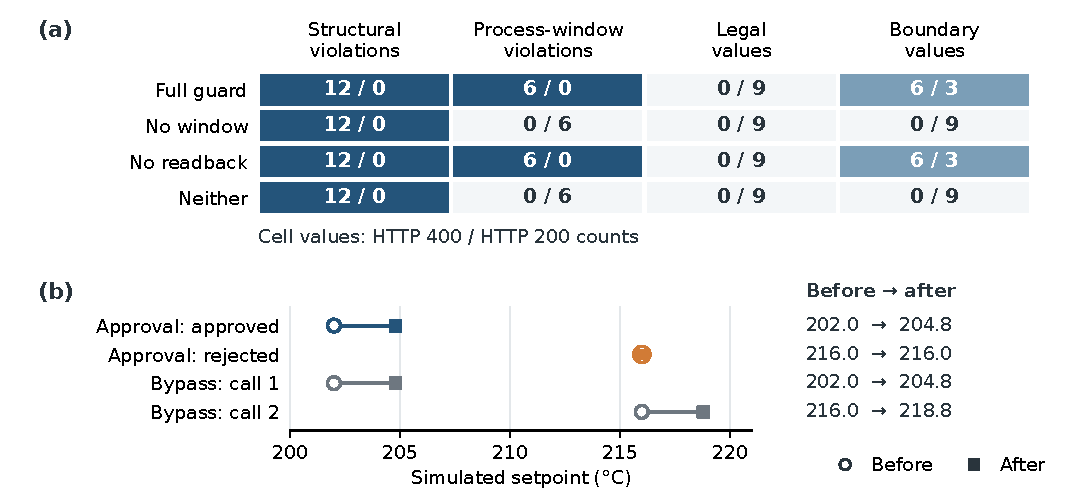
\includegraphics[width=\textwidth]{resources/fig6.pdf}
\caption{Guard-path comparison and scripted approval-route results. (a) Counts of HTTP~400 and HTTP~200 responses for four guard configurations and four request classes, with three repetitions per configuration. Each cell lists rejected/accepted counts, and their sum is the class total; shading represents the proportion of HTTP~400 responses. The specific violation values and boundary expectations differed across configurations. The comparison did not stimulate a readback mismatch. (b) Recorded before and after simulated setpoints for four separate calls; open circles mark before and filled squares after. A scripted proxy supplied the approval decisions, and the bypass calls required no approval. The calls are not matched pairs. HTTP~200 does not establish driver dispatch.}
\label{fig:guard-approval-results}
\end{figure*}

\subsection{Injection-Twin Demonstration}
\label{sec:eval-twin-pilot}
An acceptance script ran one experiment on a PLC-based simulated twin (\texttt{realPlant=false}). A governed write changed the setpoint from 60 to 63.7~bar, the simulated readback matched, and three later samples averaged 32.224~g after the specified wait. The structured baseline is 31.503~g, whereas the report states 31.508~g; the discrepancy and missing raw sample series and runtime snapshot prevent this run from supporting an effect estimate.

\subsection{LLM-Driven Simulator Episodes}
\label{sec:eval-agent}
Three LLM-driven injection episodes ended \texttt{CANCELED} below the 32.15--32.85~g band, at 31.70, 31.87, and 31.99~g. The saved worker label is a blinded model label, and the served model version is absent. Each worker trace records one \texttt{recipe\_trial} call to update two setpoints and a response reporting both as acknowledged; approval was automatic, and one episode carries a guard-violation flag. The row-level server journal was not retained, so these responses do not independently verify driver dispatch. The episodes do not estimate agent success, operator approval effects, or physical execution.

